% About 2 pages
% Survey of existing work on the problems that this project addresses (lit review).

\subsection{MAC randomisation and 802.11 fingerprinting}\label{sec:mac-randomisation-lit}

There have been many attempts at either overcoming or to point out the flaws with MAC randomisation.
The majority of its literature appears post-2015, around the time of its widespread introduction.

~\citeasnoun{Pang2007} were ahead of their time when they presented a technique which is able to uniquely identify devices without the need for a MAC address.
This type of technique will be referred to as \emph{implicit identifier fingerprinting}.
Because it yields good results, the method is selected as one of the methods to be used in the hybrid system.
However, due the continued maturing of the 802.11 protocol and improved manufacturing techniques, it should be expected that tolerances on the previously discussed fields become more narrow over time.
Hence, consideration should be taken into account about how the different 802.11 versions affect both the hybrid system and implicit identifier fingerprinting.
This forms the motivation behind the third objective question and is discussed further in Section~\ref{sec:solution}.

~\citeasnoun{Vanhoef2016} perform a technical breakdown of several novel techniques to track mobile devices, bypassing MAC randomisation.
It was one of the first papers to specifically aim at bypassing MAC randomisation.
One such technique involves looking up one of the WPS fields (the Universally Unique IDentifier-Enrolle (UUID-E)) in a hash table to retrieve the true MAC address.
One of the datasets they used was~\cite{barbera2013crawdad}, issues have been pointed out in their analysis pertaining to the fact this dataset was anonymised and there was no ground true to validate against, leading to questions being asked about the integrity of the paper and methods presented, especially given MAC address randomisation was not rarely implemented in 2013.

\citeasnoun{Martin2017} assessed the effectiveness of MAC randomisation and performed a critical evaluation of~\citeasnoun{Vanhoef2016}.
As part of this, they produced their own dataset to better represent probe requests sent by modern devices, and more importantly those including MAC randomisation.
They then improved on the fingerprinting technique presented by~\cite{Vanhoef2016}, being able to effectively defeat MAC randomisation in about 96\% of Android phones.
Finally, they presented a new physical-layer flaw which enables, under various circumstances, an active attack able to track any of the devices they tested.
\citeasnoun{fenske2021} follows-up on~\cite{Martin2017} by experimentally testing MAC randomisation on 160 mobile phone models and found that many of them still do not implement adequate MAC randomisation -- they still emit implicit identifiers (primarily divided by device make and model).
In particular, they conclude that some relatively modern android devices are particularly inconsistent with the MAC randomisation they provide, leaving them strongly susceptible to the implicit identifier fingerprinting attacks.
Importantly, they note that the older attacks which are able to recover the true MAC address have been largely phased out.

In parallel to~\cite{Vanhoef2016},~\citeasnoun{Matte2016} present a novel timing-based attack.
This works by statistically analysing and grouping, by device, sets of probe request frames transmitted over time using their IAT.
Ultimately, this collects a dictionary of MAC addresses used by the device and has seen success with tracking multiple devices over time.
For their PhD thesis,~\citeasnoun{matte2017} performed an in-depth review of 802.11 fingerprinting, expanding on their 2016 timing attack and improving on implicit identifier fingerprinting.

In addition to the previously mentioned MAC vendor analysis which works at the data-link layer,~\citeasnoun{robyns2017} provides two more data-link layer vulnerabilities.
The first technique fingerprints a device transmitter by performing per-bit entropy analysis.
The other uses temporal information in a similar way to that of~\cite{Matte2016}.
With this, they produce a dataset consisting of \~30,000 unique devices (taken from an outdoor festival) and show the first technique to be capable of successfully fingerprinting 80\% of 50 and 68\% of 100 observed devices.
For 1,000 to 10,000 devices, performance degrades considerably to a 33\% to 15\% success rate respectively.

MAC addresses consist of six octets, for universal MAC addresses the first three bytes of which uniquely identify the manufacturer (an organisationally unique identifier) and the last three bytes are uniquely assigned by the manufacturer.
Here, the second-least significant bit of the third octet, referred to as the locally administered (LA) bit, is always zero.
When this bit is set to one, the address becomes an LA MAC address.
For 802.11 to work, this must be unique within a local area network (LAN) but otherwise may be freely chosen by the operating system.
This is demonstrated in Figure~\ref{fig:mac-address}.
As a continuation of their PhD work,~\citeasnoun{Matte2018} use this to study the spread of MAC randomisation in probe request datasets spanning between 2013 and 2017 by checking if addresses have the LA bit set.
This is helpful because it considers data from both before adoption of MAC randomisation, by including the~\cite{barbera2013crawdad} dataset, and after, by using datasets such as those provided by~\cite{Martin2017} and~\cite{robyns2017}.
The study comes to an interesting conclusion stating that, where there is a steady increase in usage of MAC randomisation, only 3\% of probe requests (as of the 2017 dataset) had the LA bit set.
Since it is such a fast-moving field however, with the recent releases of iOS 14 and Android 10, an updated study is required.
This lack of modern (post 2020 indoor) data is part of the motivation behind the development of the data simulation framework.

\begin{figure}[!ht]
    \centering
    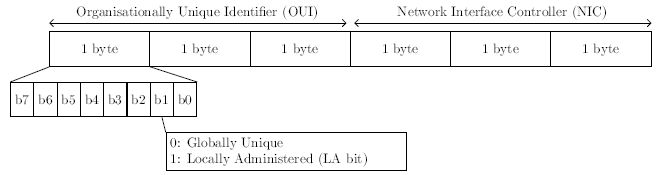
\includegraphics[scale=0.6]{figures/macaddress.png}
    \caption{Format of a MAC address from \protect\cite{Matte2018}.}
    \label{fig:mac-address}
\end{figure}

\subsection{Privacy and Ethical Issues}\label{sec:privacy-issues}

An inherent problem with LBSs is that of preserving user privacy while still making meaningful use of them.
The timestamped location (spatio-temporal information) of a person is generally considered to be very personal information.
Because of this, as long as LBSs have existed, there has been research into how privacy can be either guaranteed or personalised by the user.
From a technical standpoint, this is also important to consider because the measures employed to provide anonymisation may adversely affect the ability to fingerprint.
Within the scope of this paper, it is important to take these into consideration for the design of the testing and evaluation framework.

Most privacy measures focus on LBSs that gain access to the data collected by IPSs.
This exchange is typically achieved using third party trusted middleware which anonymises data before handing it off to the end-user LBS.
~\citeasnoun{Ghinita2008} takes a more mathematical approach, employing theoretical Private Information Retrieval to anonymise positioning data returned to LBS queries. 
An added benefit of this framework is that middleware is no longer required.
Alternatively, the IPS may wish to improve privacy by slightly adjusting localisations such that they average out to a true representation, yet provide anonymity on the individual level~\cite{Kido2005}.
~\citeasnoun{Gedik2005} and~\citeasnoun{Gedik2008} propose a user-oriented approach to privacy by presenting a framework enabling the user to configure the amount of anonymity it desires, in addition to their desired spatio-temporal resolution.
Finally, an alternative to passive user tracking worth briefly mentioning is that proposed in~\cite{Furfari2021}.
This would mitigate the discussed privacy issues by enabling users to opt-in to discovering location-based services, at which point they give permission to access their location data.
From this, the best and simplest privacy measure for simulation of real-world data is the trusted middleware model.
Aside from the fact the data is not real, this stops the emulated IPS from having to consider privacy, better enabling it to generalise.
